\section{Durchführung}

\subsection{Fourier-Synthese}
Um die verschiedene Funktionen zu synthetisieren, wird mit einem Multimeter die Grundspannung $U_0=\qty{0.5}{\volt}$ gemessen.
Damit die Amplituden der einzelnen Oberwellen eingestellt werden, werden diese zuerst berechnet.
Diese werden dann als Vielfaches der Grundspannung eingestellt.
Ein Oberwellengenerator wird nun mit der Grund- und jeweils einer der Oberschwingungen, an das Oszilloskop angeschlossen.
Dieses wird auf x-y Betrieb eingestellt.
Danach wird die Phase der Oberschwingungen so eingestellt, dass eine Lissjaous-Figur zu sehen ist.
Dies erfolgt für alle Oberschwingungen.
Weitere Anpassungen erfolgen im Nachhinein, indem die Schalter für Phasenverschiebungen um $\frac{\pi}{2}$ und $\pi$ so betätigt werden, sodass die am Oszilloskop abgebildete Funktion die Gegebene bestmöglich annähert.

\label{sec:Durchführung}
\subsubsection{Amplituden der Rechteckspannung}
Die Rechteckspannung ist hier als ungerade Funktion definiert.
Daher müssen bei der Beschreibung mit einer Fourier-Reihe, die sich aus Formel \ref{eqn:reihe} ergibt, die Koeffizienten $a_n$ nicht berücksichtigt werden.
Für die anderen Koeffizienten gilt Formel \ref{eqn:b_n}.
Durch Einsetzen und Integrieren ergibt sich 
\begin{equation*}
    b_n=\frac{4a}{\pi n} \qquad n\in2k+1 \; k\in\mathbb{N}
    \label{eqn:amp_recht}
\end{equation*}
für die Amplituden und damit folgt
\begin{equation*}
    f(t)=\sum_{n=1}^{\infty}\Bigl( \frac{4a}{\pi n} \symbf{sin}(n t)\Bigr) 
    \label{eqn:recht}
\end{equation*}
für die Fourier-Reihe der Rechteckspannung.
Der Betrag der Amplituden entspricht
\begin{equation}
    |b_n|=\frac{|b_1|}{n}
    \label{eqn:b_recht}
\end{equation}.
Damit ist das benötigte Verhältnis der Oberwellen zur Grundwelle $\frac{1}{n}$ zu 1.
Wegen der Einschränkungen für n können die geraden Oberwellen vernachlässigt werden.
%%Bilder und Beträge eingügen

\subsubsection{Amplituden der Dreieckspannung}
Bei der Dreieckspannung wird auch diese so definiert, dass die Funktion ungerade ist.
Die Berechnung erfolgt daher wie oben mit den Formeln \ref{eqn:reihe} und \ref{eqn:b_n}.
Daher sind die Koeffizienten
\begin{equation*}
    b_n=(-1)^k\frac{4a}{\pi n^2} \qquad n\in2k+1 \; k\in\mathbb{N}
    \label{eqn:amp_drei}
\end{equation*}   
und die Funktion entspricht
\begin{equation*}
    f(t)=\sum_{n=1}^{\infty}\Bigl((-1)^k \frac{4a}{ \pi n^2} \symbf{sin}(n t)\Bigr) 
    \label{eqn:drei}
\end{equation*}.
Für den Betrag der Koeffizienten gilt
\begin{equation}
    |b_n|=\frac{|b_1|}{n^2}
    \label{eqn:b_drei}
\end{equation}.
Daher muss für die Amplituden der Oberwellen die der Grundwelle mit $\frac{1}{n^2}$ multipliziert werden. 
Aufgrund der Einschränkungen für n werden nur die ungeraden Oberschwingungen berücksichtigt.

\subsubsection{Amplituden der Sägezahnspannung}
Auch bei der Sägezahnspannung kann diese ungerade definiert werden.
Analog zu den Berechnungen oben folgt
\begin{equation*}
    b_n=(-1)^{n+1}\frac{2a}{ n} \qquad n\in\mathbb{N}
    \label{eqn:amp_säge}
\end{equation*} 
für die Amplituden und für die Funktion
\begin{equation*}
    f(t)=\sum_{n=1}^{\infty}\Bigl( (-1)^{n+1}\frac{2a}{ n} \symbf{sin}(n t)\Bigr) 
    \label{eqn:drei}
\end{equation*}.
Der Betrag der Amplituden wird mit
\begin{equation}
    |b_n|=\frac{|b_1|}{n} 
    \label{eqn:b_säge}
\end{equation}
berechnet. Damit ist das Verhältnis hier dasselbe, wie bei der Rechteckspannung.

\subsection{Fourier-Analyse}
Für die Analyse wurde ein Signalgenerator an das Oszilloskop wie in Abbildung \ref{fig:analyse} angeschlossen.

% \begin{figure}
%     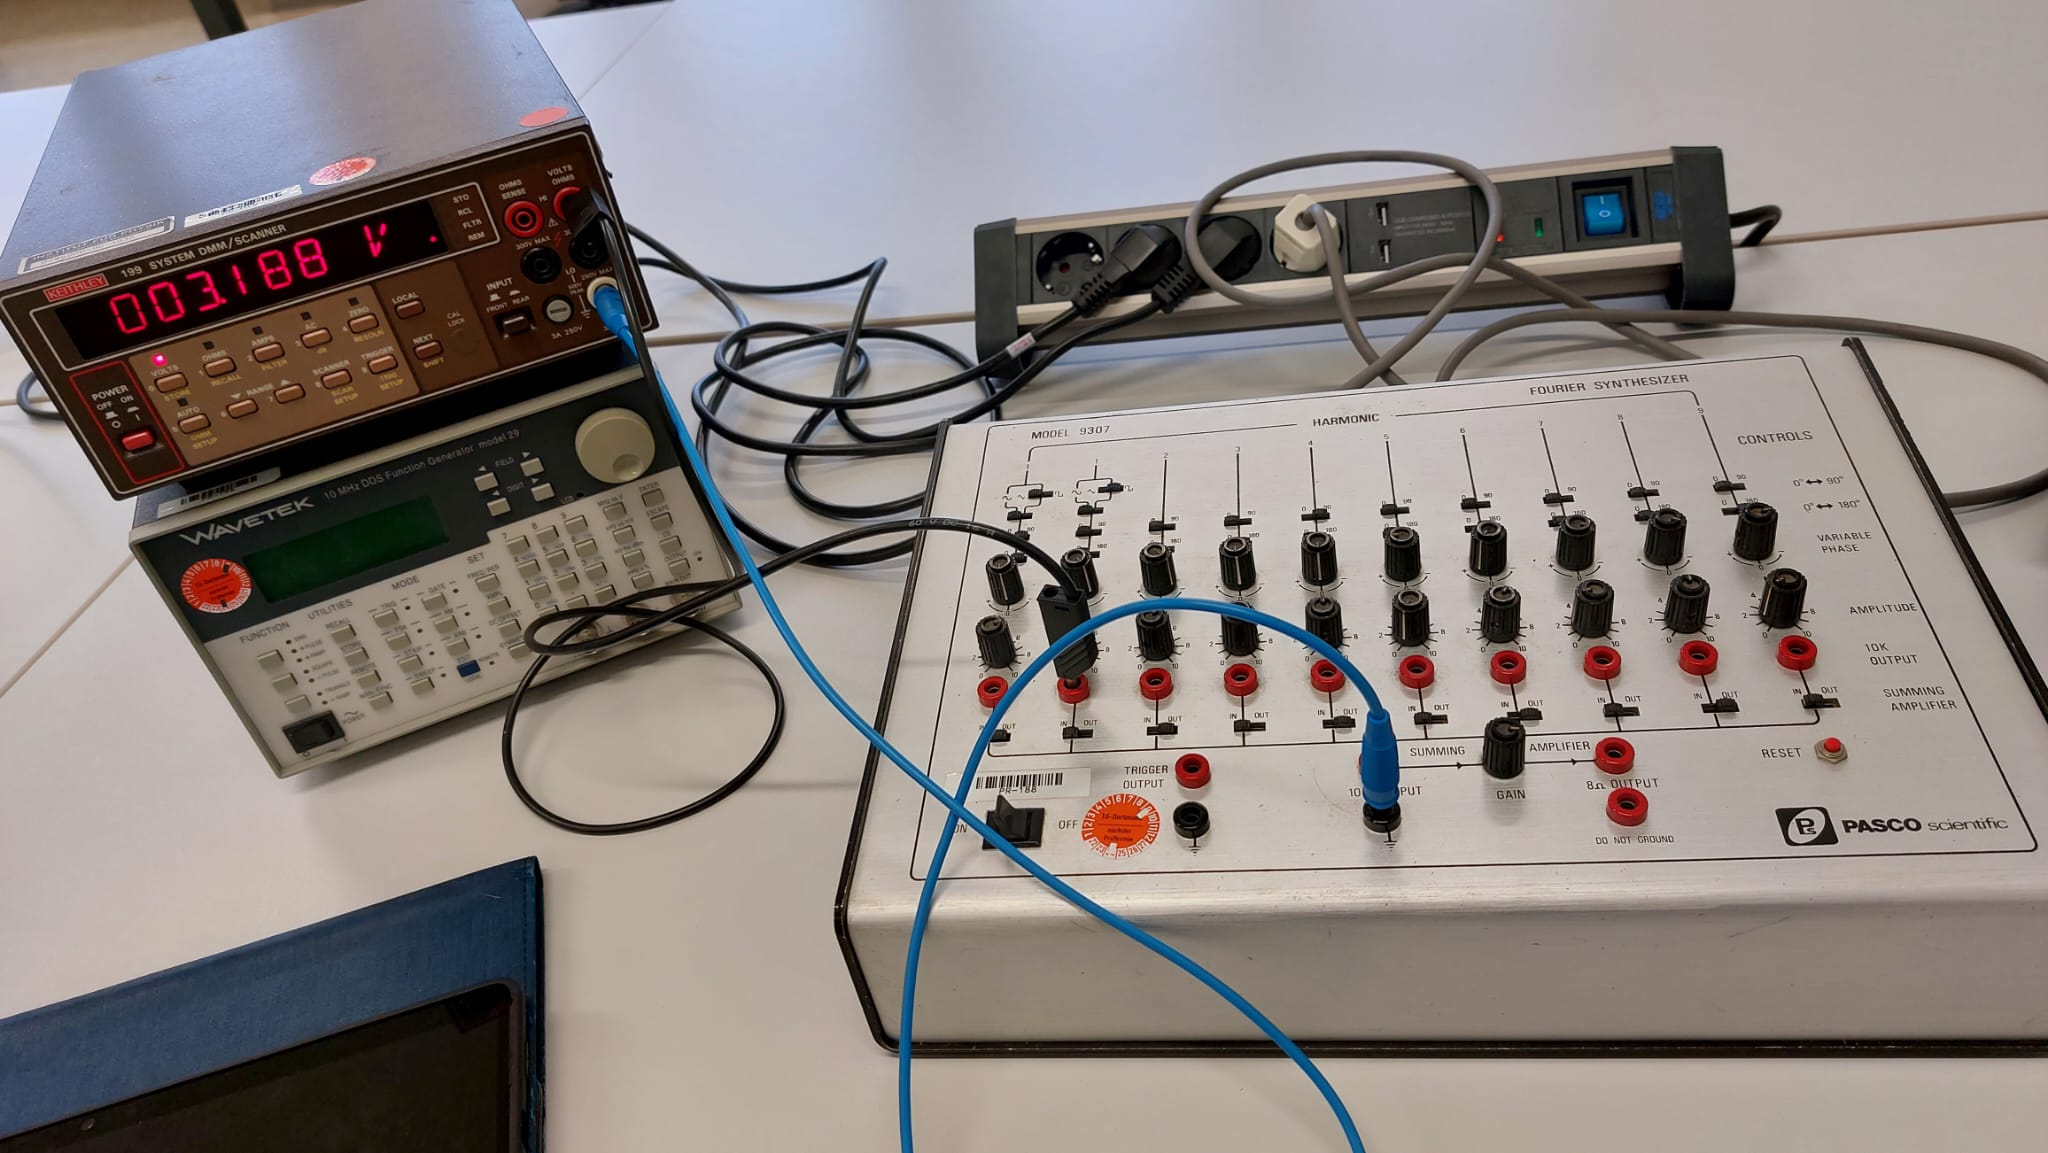
\includegraphics{Bilder/synthese.jpg}
%     \label{fig:synthese}
%     \caption{Abgebildet ist der Aufbau für das Einstellen der Oberschwingungen.}
% \end{figure}
% 
% \begin{figure}
%     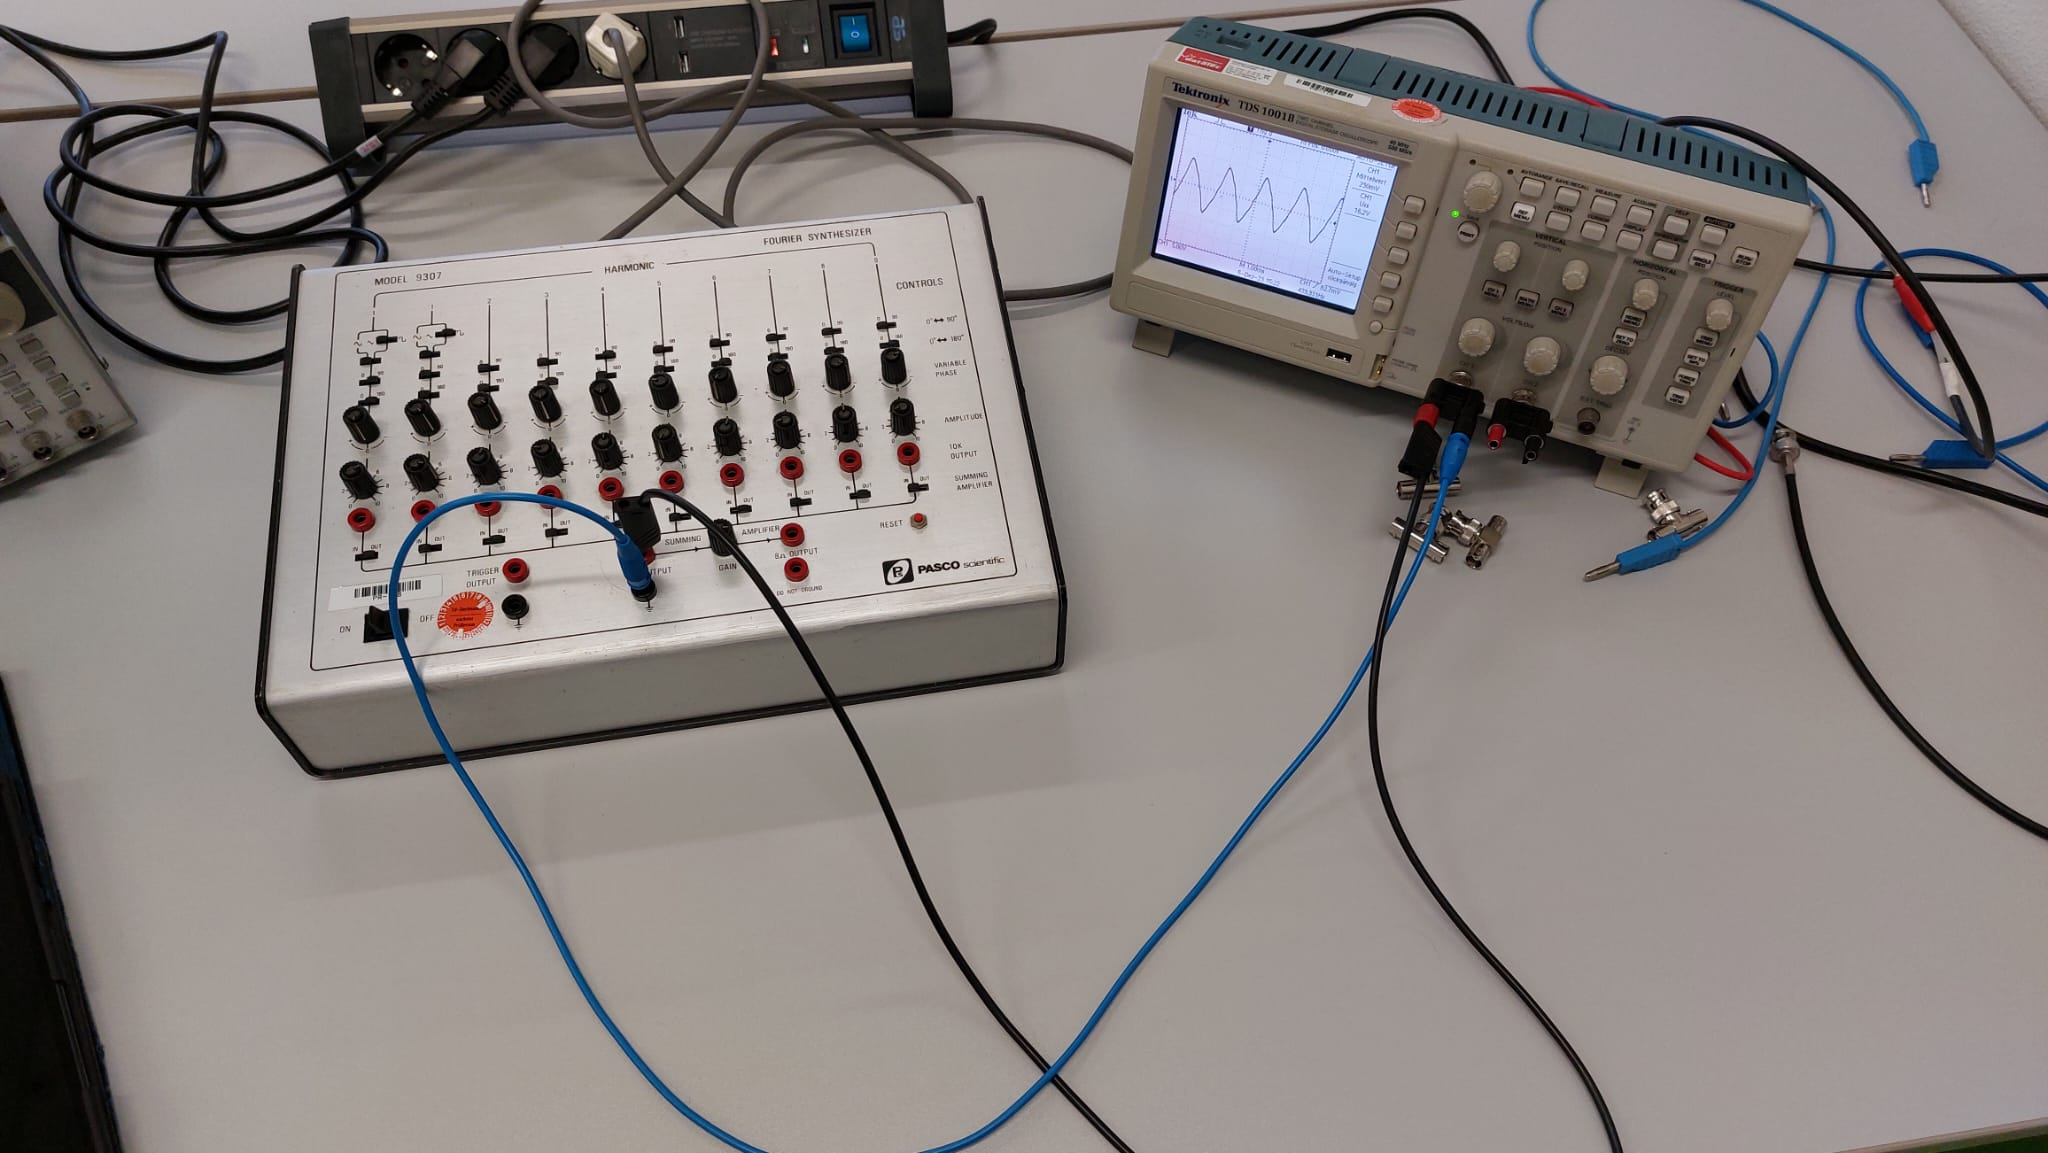
\includegraphics{Bilder/synthese2.jpg}
%     \label{fig:synthese2}
%     \caption{Abgebildet ist der Aufbau für das Einstellen der Oberschwingungen.}
% \end{figure}

\begin{figure}[H]
    \includegraphics[width=\textwidth]{Bilder/analyse.jpg}
    \label{fig:analyse}
    \caption{Abgebildet ist der Aufbau für die Fourier-Analyse.}
\end{figure}

Das Oszilloskop führt, mit der richtigen Einstellung, eine Fouriertransformation durch.
Von dem angezeigten Graphen, auf welchem die Amplituden der Oberwellen in Abhängigkeit zur Frequenz aufgetragen sind, werden dann die Werte bei den Peaks gemessen.

